
\section{A New Resilience Metric for Production Networks} \label{sec:architectures}

The fact that power laws can arise in supply chain graphs, as we show in \cref{theorem:power_laws}, yields the need to define a resilience metric. It is important to have a proper metric for resilience to understand the behavior of complex systems and identify potential vulnerabilities. There are many different ways to define and measure resilience, and which metric is most appropriate will depend on the specific system being studied and the goals of the analysis. Some common approaches to defining resilience include looking at the system's ability to recover from disturbances, absorb or adapt to change, and maintain function in the face of stress or disruption.


In our percolation model, ideally, a ``more resilient'' network is a network that can withstand larger productivity shocks, which are associated with larger percolation probabilities $x$. Therefore, it is natural to assume that in a resilient network, we want to find the maximum value that the percolation probability $x$ can get in order for a ``large'' fraction of the items to survive almost surely. Formally, for $\varepsilon \in (0, 1)$, the \emph{resilience} of a (possibly random) product graph $\cG$ is defined as 
$$R_{\cG} (\varepsilon) = \sup \left \{ x \in (0, 1) : \Pr_{\cG,x} { \left [S \ge (1 - \varepsilon)  {K} \right ]} \ge 1 - \frac {1} {\ev {\cG} {K}} \right \},$$
%\mar{Can we write this in terms of the joint distribution (x and G)? $\Pr_{\cG,x} \left[S \ge (1 - \varepsilon) {K}  \ge 1 - \frac {1} {{K}}\right]$} 
and corresponds to the maximum percolation probability for which at most $\varepsilon K$ products fail with high probability. The expectation $\ev {\cG} {\cdot}$ corresponds to the randomness of the graph generation process, and the probability $\Pr_{\cG, x} [\cdot]$ corresponds to the joint randomness of the percolation and the graph where the randomness of the graph can be over the nodes, the edges, or both. In the case of $\mathsf{rdag}(K, p)$, our lower bound on $x$ in Appendix \ref{app:analytical_lower_bound} for ensuring $\Pr [F \ge \varepsilon K] = O(1/K)$ is also a lower bound on the resilience for this particular architecture. 

We are interested in the following questions: Do supply chains $\cG$ for which $R_{\cG} \to 0$ as $K \to \infty$ exist? Do supply chains $\cG$ for which $R_{\cG} \to R$ for some $R \in (0, 1]$ as $K \to \infty$ exist? The former type of architecture can be characterized as a \emph{fragile architecture} since even the tiniest failure can devastate the network. The latter one can be characterized as a \emph{resilient architecture} since it can withstand non-trivial shocks in the limit of $K \to \infty$. 

% \mpcomment{add table for resiliency results here}

In the sequel, we study a variety of network architectures and derive lower bounds for the resilience of such supply chain architectures. \cref{tab:resiliences} summarizes our results. Briefly, in order to prove that a supply chain $\cG$ is resilient it suffices to choose some percolation probability $\underline R_{\cG}(\varepsilon) \in (0, 1)$ such that $\Pr_{x = \underline R_{\cG}(\varepsilon)} [F \ge \varepsilon K] = O \left ( {1}/{K} \right )$ and prove that $\lim_{K \to \infty} \underline R_{\cG}(\varepsilon) > 0$, which implies that $\lim_{K \to \infty} R_\cG(\varepsilon) > 0$ since $R_{\cG}(\varepsilon) \ge \underline R_{\cG}(\varepsilon)$. Moreover, to prove that architecture is fragile, we prove an upper bound $\overline R_{\cG}(\varepsilon) \in (0, 1)$ on the resilience and show that this upper bound goes to 0 as $K \to \infty$. In order to derive upper bounds, we can use the following Lemma, whose proof is deferred in Appendix \ref{app:proof:upper_bound_resilience}. The $1/2$ constant below is arbitrary and the proof works for any constant $\theta \in (0, 1)$.

\begin{lemma} \label{lemma:upper_bound_resilience}
    Let $\varepsilon \in (0, 1)$ and let $\overline R_{\cG}(\varepsilon) \in (0, 1)$ be a percolation probability such that $\Pr_{x = \overline R_{\cG}(\varepsilon)} [S \ge (1 - \varepsilon) K] \le \frac 1 2$. Then, for $K \ge 3$, we have that $\overline R_{\cG}(\varepsilon) > R_{\cG}(\varepsilon)$. 
\end{lemma}

As a warmup, the analysis of \cref{sec:motivation} shows that $\mathsf{rdag}(K, p)$ is a fragile architecture, and therefore, we get our first theorem:

\begin{theorem} \label{theorem:rdag_resilience}
    Let $\cG \sim \mathsf{rdag}(K, p)$. Then, as $K \to \infty$, we have that $R_{\cG} (\varepsilon) \to 0$.
\end{theorem}

% \begin{proofsketch}
%     See the analysis in \cref{sec:motivation}. 
% \end{proofsketch}

In the next Sections, we study various architectures and derive upper and lower bounds of $R_{\cG}(\varepsilon)$. 

\subsection{Parallel Products with Dependencies} \label{sec:parallel_products}


\begin{figure}[t]
    \centering
    \subfigure[$\mathsf{rdag}(K = 3, p)$\label{fig:random_dag_2}]{
    \begin{tikzpicture}[transform shape]
        \Vertex[x=-2, y=0, label=$1$, color=pink]{u1}
        \Vertex[x=0, y=0, label=$2$]{u2}
        \Vertex[x=2, y=0, label=$3$, color=pink]{u3}
        \Edge[Direct, color=black, label=$1- p$, style={dashed}](u1)(u2)
        \Edge[Direct, color=black, label=$p$, ](u2)(u3)
        \Edge[Direct, color=black, label=$p$, bend=30](u1)(u3) 
    \end{tikzpicture}} \quad
    \subfigure[Parallel Products ($d = 2$, $m = 3$).\label{fig:parallel_products}]{
    \begin{tikzpicture}[]
        \Vertex[x=-0.25,y=0,Pseudo,label={$\cR$}]{r0}
        \Vertex[x=4.25,y=0,Pseudo]{x}

        \Vertex[x=1,y=0,color=pink]{r1}
        \Vertex[x=2,y=0]{r2}
        \Vertex[x=3,y=0]{r3}

        \Vertex[x=-0.25,y=1.25,Pseudo,label={$\cC$}]{c0}

        \Vertex[x=1,y=1.25,color=pink]{c1}
        \Vertex[x=2,y=1.25,color=pink]{c2}
        \Vertex[x=3,y=1.25]{c3}  

        \Edge[color=black,Direct](r1)(c1)
        \Edge[color=black,Direct](r1)(c2)
        \Edge[color=black,Direct](r2)(c2)
        \Edge[color=black,Direct](r2)(c3)
        \Edge[color=black,Direct](r3)(c3)
        \Edge[color=black,Direct](r3)(c1)
        
    \end{tikzpicture}}
    
    %\shrink
    \caption{Production networks of \cref{sec:motivation} and \cref{sec:parallel_products}. Failures are drawn in pink color.}
    \shrink
    \label{fig:parallel_products_rdag}
\end{figure}


The first architecture we study is parallel products. Here we aim to produce $K$ complex products, which we denote by $\cC$, and each complex product requires $|\cN(i)| = m$ inputs (raw materials; source dependencies) to be produced. The set of raw materials (denoted by $\cR$) contains $|\cR| = \rho$ raw materials. We further introduce supply dependencies among the raw materials by assuming that each raw material can supply $d$ products. \cref{fig:parallel_products} shows an example of such a supply chain together with an instance of the percolation process (affected nodes are drawn in pink). Here it is interesting to study both the resilience of the whole graph, i.e., the graph with vertex set $\cC \cup \cR$, as well as the resilience of the complex products $\cC$ alone. We show that if the source dependency $m$ and the supply dependency $d$ between the products is bounded, then the production network is resilient. The resilience metric is lower-bounded by $\left ( \frac {\varepsilon} {2(d+1)m} \right )^{1/n}$ in both cases (complex products alone or together with raw materials), as the number of products goes to infinity. Moreover, if the number of inputs $m$ goes to infinity, the resilience of the whole graph goes to $0$ at rate $O \left ( e^{- \frac {1} {mn}} \right )$, and the resilience of the complex products goes to $0$ at rate $O \left ( e^{- {c^{\frac 1 m}}/{n}} \right )$ for some constant $c \in (0, 1)$. Formally, we prove the following for the resilience of the parallel products: 

% \mpcomment{Make theorems consistent and have only UB and LB there, + case when $K \to \infty$. Give intuitive explainations about the rates.}

\begin{theorem} \label{theorem:parallel_products}
    Let $\cG$ consist of $K$ parallel products and assume that these products can be produced by $|\cR| = \rho$ raw materials, and each material is used by at most $d$ products. The resilience of the complex products $\cC$ satisfies:
    $\left ( \frac {\varepsilon} {dm} + \sqrt {\frac {\log K} {2mK}} \right )^{1/n} \le R_{\cC}(\varepsilon) \le \left ( 1 - \left ( \frac {1 - \varepsilon} 2 \right )^{1/m} \right )^{1/n}$. Also, the resilience of all products satisfies: $\left ( \frac {\varepsilon} {2 (d + 1)m} + \sqrt {\frac {\log (K/2)} {2mK}} \right )^{1/n} \le R_{\cG}(\varepsilon) \le \left ( 1 - \frac {1 - \varepsilon} {2 (m + 1)} \right )^{1/n}$. Subsequently, if $\varepsilon, d$ and $m$ are independent of $K$, then then the resilience is $\Omega \left ( \left ( \frac {\varepsilon} {dm} \right )^{1/n} \right )$ as $K \to \infty$. 
\end{theorem}

\begin{proofsketch}
    For brevity, we give an analysis in expectation for $R_{\cC}(\varepsilon)$. The high-probability analysis has been deferred to Appendix \ref{app:proof:theorem:parallel_products}, where the lower bound is improved by an additive factor of $\sqrt{\frac {\log K} {2mK}}$ via Chernoff bounds. The analysis for $\cG$ is similar. To show the lower bound, we show that to have at least $\varepsilon K$ complex products fail in total, we need at least $\varepsilon K/d$ raw materials to fail. The expected number of raw materials that fail is $\rho x^n \le m K x^n$, and therefore by equating $\frac {\varepsilon K} d$ with $mKx^n$, we get the desired answer. To derive the upper bounds, we simply upper bound the expected number of surviving complex products $\ev {} {S_{\cC}} = K(1 - x^n)^m$ and apply Markov's inequality and \cref{lemma:upper_bound_resilience}.
\end{proofsketch}
\subsubsection*{Additional Results.} In Appendix \ref{app:random_trellis}, we analyze the resilience of a random width-$w$ trellis graph width $D$ tiers (and $K = wD$ nodes) where edges between subsequent tiers are generated i.i.d. with probability $p$, which can be thought of as an extension to the parallel products' architecture. In \cref{theorem:trellis_resilience}, we discover an interesting ``duality phenomenon''; i.e., when $pw \le 1$ a constant depth random trellis resilient, and when $pw \ge 1$ a constant width trellis is fragile.  

% \mar{trellis insights}
% Moreover, if $d = 1$, we can improve the lower bound of the resilience of the parallel products and show that the resilience admits an exponential improvement. The analysis is deferred in the Appendix and relies on a simple application of the Chernoff bound. 

% \begin{proposition} \label{theorem:parallel_one_resilience}
%     Let $\cG$ consist of $K$ products where each product has $m$ inputs, each input consists of $n$ suppliers, and each raw material is used by exactly $d = 1$ product. Then $R_{\cC} \ge \left ( 1 - \left  (1 - \varepsilon + \sqrt{\frac {\log K} {2K}} \right )^{1/m} \right )^{1/n}$. Subsequently, as $K \to \infty$ we have that $R_{\cG}(\varepsilon) \ge \left ( 1 - e^{-\frac {\varepsilon} {m}} \right )^{1/n}$ for $m, n, \varepsilon$ independent of $K$.
% \end{proposition}

% \begin{proofsketch}
%     The number of successfully produced complex products is a binomial variable with $K$ trials and success probability $(1 - x^n)^m$. By using standard Chernoff bounds for bounding the probability that $S_{\cC} \ge (1 - \varepsilon) K$ we get the desired result. 
% \end{proofsketch}

% \begin{proof}
%     The probability of each product being produced is $(1 - x^n)^m$, and the number of products produced follows a binomial distribution with $K$ trials and probability of success $(1 - x^n)^m$. From the Chernoff bound, we get that $\Pr [S_{\cC} \ge (1 - \varepsilon)K] \ge 1 - e^{-2K (1 - (1 - x^n)^m - \varepsilon)^2}$. We set the above probability to be $1 - 1 / K$, which yields 

%     \begin{align*}
%         x = \left ( 1 - \left  (1 - \varepsilon + \sqrt{\frac {\log K} {2K}} \right )^{1/m} \right )^{1/n}
%     \end{align*}
   
    
%     Thus we get that the resiliency of the parallel products is $R_{\cC}(\varepsilon) \ge \left ( 1 - \left  (1 - \varepsilon + \sqrt{\frac {\log K} {2K}} \right )^{1/m} \right )^{1/n}$. For $K \to \infty$, and $m, n, \varepsilon$ independent of $K$, we have that $R_{\cC}(\varepsilon) \to (1 - (1 - \varepsilon)^{1/m})^{1/n}$. Using the convexity of $e^t$ we get that as $K \to \infty$, the resilience is at least $\left ( 1 - e^{-\frac {\varepsilon} {m}} \right )^{1/n}$.
% \end{proof}

\subsection{Hierarchical Production Networks}

A supply chain can be organized hierarchically, with different levels representing different stages of the production process. The raw materials or components that go into the production of a product are at the bottom of the hierarchy, and the finished product is at the top. Each level of the hierarchy represents a stage of production where the materials or components are transformed into a more advanced or finished product \citep{elliott2022supply}. This hierarchical structure helps to visualize the flow of materials and information through the supply chain and identify potential bottlenecks or inefficiencies. Moreover, another hierarchy that is possible is producing complex products by starting from a source of raw products. In this section, we study these two hierarchies, which we call \emph{backward} and \emph{forward} (referring to the directions of the percolation with respect to the network growth), production networks visualized in \cref{fig:tree_percolation}. More specifically, we consider:
\begin{compactitem}
    \item The \emph{backward production network} (\cref{subfig:forward_backward}) at which the tree grows from the root, and then the percolation starts from the leaves and proceeds to the root. For the scope of this paper, we study backward percolation in deterministic $m$-ary trees. In \cref{sec:forward_backward_tree} we prove that, as someone would expect, such supply chains are, in fact, fragile and give lower bounds on resilience. 
    \item The \emph{forward production network} (\cref{subfig:forward_forward}) at which the tree grows from the root, and then the percolation starts from the root and proceeds to the leaves. Here, the production network is generated by a stochastic \emph{branching process}; the Galton-Watson process. In \cref{sec:forward_forward_tree}, we prove that, under specific conditions, such supply chains are fragile with a non-negative probability and are otherwise resilient.  
\end{compactitem}

\begin{figure}[t]
    \centering
    \subfigure[\label{subfig:forward_backward}]{
    \begin{tikzpicture}[transform shape, scale=0.75]
        \Vertex[x=0, y=0, color=pink]{u1}
        \Vertex[x=1, y=0.5, color=pink]{u3}
        \Vertex[x=1, y=-0.5]{u2}
        \Vertex[x=2, y=-1.5]{u4}
        \Vertex[x=2, y=-0.5]{u5}
        \Vertex[x=2, y=0.5, color=pink]{u6}
        \Vertex[x=2, y=1.5, color=pink]{u7}

        \Edge[color=black, Direct](u2)(u1)
        \Edge[color=black, Direct](u3)(u1)
        \Edge[color=black, Direct](u4)(u2)
        \Edge[color=black, Direct](u5)(u2)
        \Edge[color=black, Direct](u6)(u3)
        \Edge[color=black, Direct](u7)(u3)

        \Vertex[x=-2, y=-2, Pseudo]{x1}
        \Vertex[x=3.5, y=-2, Pseudo]{x2}
        \Vertex[x=-2, y=2, Pseudo]{y1}
        \Vertex[x=3.5, y=2, Pseudo]{y2}

        \Edge[color=blue, Direct, label={Tree Growth}](x1)(x2)
        \Edge[color=red, Direct, label={Percolation}](y2)(y1)

        
    \end{tikzpicture}} 
    \subfigure[\label{subfig:forward_forward}]{
    \begin{tikzpicture}[transform shape, scale=0.75]

        \Vertex[x=0, y=0]{u1}
        \Vertex[x=1, y=0.5]{u3}
        \Vertex[x=1, y=-0.5, color=pink]{u2}
        \Vertex[x=2, y=-1.5, color=pink]{u4}
        \Vertex[x=2, y=-0.5, color=pink]{u5}
        % \Vertex[x=2, y=0.5, color=pink]{u6}
        % \Vertex[x=2, y=1.5, color=pink]{u7}

        \Edge[color=black, Direct](u1)(u2)
        \Edge[color=black, Direct](u1)(u3)
        \Edge[color=black, Direct](u2)(u4)
        \Edge[color=black, Direct](u2)(u5)
        % \Edge[color=black, Direct](u3)(u6)
        % \Edge[color=black, Direct](u3)(u7)

        \Vertex[x=-2, y=-2, Pseudo]{x1}
        \Vertex[x=3.5, y=-2, Pseudo]{x2}
        \Vertex[x=-2, y=2, Pseudo]{y1}
        \Vertex[x=3.5, y=2, Pseudo]{y2}

        \Edge[color=blue, Direct, label={Tree Growth}](x1)(x2)
        \Edge[color=red, Direct, label={Percolation}](y1)(y2)
    \end{tikzpicture}}
    \subfigure[\label{fig:gw_subcritical}]{\includegraphics[width=0.3\textwidth]{figures/gw_resilience_subcritical.pdf}}
    %\shrink
    
    \caption{(a, b): Backward and Forward Networks. Node failures are drawn in pink. (c): Resilience bounds for a subcritical GW process with branching distribution as a function of $\mu$; note the decreasing trends in both upper and lower bounds, $\ev {\cG} {\overline R_{\cG}(\varepsilon)}$ and $\ev {\cG} {\underline R_{\cG}(\varepsilon)}$, with increasing $\mu$.}
    \label{fig:tree_percolation}
    \shrink
\end{figure}

In the sequel, we present the two processes and the results on $R_{\cG}(\varepsilon)$, and in \cref{sec:comparison_golub}, we compare our conclusions with the ones of \citet{elliott2022supply}.

\subsubsection{Backward Production Network} \label{sec:forward_backward_tree}

In the case of the backward production network, we consider an $m$-ary tree with height $D$ and fanout $m \ge 1$. The levels of the tree correspond to ``tiers'' with raw materials being positioned at tier $D$ and more complicated products positioned in higher tiers. Each product has $n$ potential suppliers, and each product at tier $d \in [D - 1]$ has exactly $|\cN(i)| = m$ inputs from tier $d + 1$. Tier $d = D$, which corresponds to the raw products, does not have any inputs. \cref{subfig:forward_backward} shows how the percolation process evolves in a tree with $m = 2$ and $D = 3$, where failures (drawn in pink) propagate from the two faulty raw materials up to the root.  

In addition to the power law result (\cref{theorem:power_laws}), the case of the $m$-ary tree is another example that motivates the resiliency measure $R_{\cG}(\varepsilon)$. Specifically, let's think about the probability of a catastrophic failure in a tree --- i.e., one that affects a substantial proportion of the suppliers in the production network. A raw material failing to be produced can cause its parent product not to be produced and inductively create a cascade up to the root. The complete cascade will start from the failed product at tier $D - 1$ since some products at tier $D - 1$ may be made if their corresponding raw materials are produced. However, no product can be produced from tier $D - 2$ and onward. As a result, only $o(K)$ products survive. The probability of such an event equals: 
\begin{align} \label{eq:quick}
    \Pr [S = o(K)]  \ge \Pr [\text{$\ge 1$ raw material malfunctions}] = 1 - (1 - x^n)^{m^{D - 1}} \ge 1 - e^{-x^n m^{D - 1}}. 
\end{align}
It is easy to see that if $x = \Omega \left ( \left ( {m \log K}/{K} \right )^{1/n} \right )$, then a catastrophe happens with a high probability in the tree structure, meaning that failure probabilities as small as  $\left (  {m \log K}/ {K} \right )^{1/n} + o(1)$ can cause catastrophes with probability approaching one (and therefore, the backward hierarchical production network is a fragile architecture). Therefore, it is interesting to study cases where such a scenario does not happen; on the contrary, we have many products surviving. The following Theorem formalizes lower bounds and provides an additional upper bound for the resilience of the backward production network. 

\begin{theorem} \label{theorem:tree_resilience}
    Let $\cG$ be a backward production network with fanout $m$ and depth $D$. Then, 
    \begin{align}
        \left [ 1 - \left ( 1 - \frac 1 {K} \right )^{\frac {1} {(1 - \varepsilon) K}} \right ]^{1/n} \le R_{\cG}(\varepsilon) \le \begin{cases}
            \left ( \frac {2} {K (1 - \varepsilon)}\right )^{1/n} = \left ( \frac {2} {D (1 - \varepsilon)}\right )^{1/n}, & m = 1 \\
            \left ( \frac {(1 - \varepsilon) \log m} {\log K} \right )^{1/n} \asymp \left ( \frac {(1 - \varepsilon)} {D} \right )^{1/n}, & m \ge 2. 
        \end{cases} 
    \end{align}

    Therefore, as $K \to \infty$ with $m$ finite, we have $R_{\cG}(\varepsilon) \to 0$. 
\end{theorem}

\begin{proofsketch}
    To derive the lower bound (for both $m = 1$ and $m \ge 2$), we show that if a failure happens at tier $\tau$, then all of the products up to tier $\tau$ have to be operational, which implies a lower bound on the tail probability of $S$, i.e., $\Pr [S \ge (1 - \varepsilon) K] \ge (1 - x^n)^{(1 - \varepsilon) K}$. To derive an upper bound, we show that when $m = 1$ then $\ev {} {S} \le 1 / x^n$, and when $m \ge 2$ we show (see Appendix \ref{app:upper_and_lower_bounds_tree}) that $\ev {} {S} \le KDx^n / 2$, and the rest follows by \cref{lemma:upper_bound_resilience}, and $D \ge \log K / \log m$ (for $m \ge 2$). 
\end{proofsketch}

\paragraph{Upper Bound Comparison.} Since $\varepsilon \in (0, 1)$ the above quantity behaves asymptotically as $O \left ( \left ( \frac {\log m} {\log K} \right )^{1/n} \right )$ for all values of $\varepsilon$. Therefore, the resilience goes to 0 with rate $\log K$. However, note that in \cref{eq:quick}, we showed a better rate of $O \left ( \left ( \frac {m\log K} {K} \right )^{1/n} \right )$, and therefore we state that the resilience goes to 0 with a rate of $O \left ( \left ( \frac {m\log K} {K} \right )^{1/n} \right )$ (for $m \ge 2$). 

% \mpcomment{explain which bound is better than other}

\subsubsection{Forward Production Network} \label{sec:forward_forward_tree}

We consider a random hierarchical network where the products in each level $d$ are denoted by $\cK_d$. Starting from one raw material $r$, i.e., $\cK_1 = \cR = \{ r \}$, we branch out via a Galton-Watson (GW) process such that every product $i \in \cK_d$ at level $d \ge 1$ creates $\xi_{i}^{(d)}$ supply dependencies, where $\{ \xi_{i}^{(d)} \}_{i \in \cK_d, d \ge 0}$ are generated i.i.d. from a distribution $\cD$, with mean $\ev {\cD} {\xi_{i}^{(d)}} = \mu > 0$. Subsequently, the number of products at each level obeys
\begin{align} \label{eq:gw_1}
    |\cK_{d + 1}| = \begin{cases} 
        \sum_{i \in \cK_d} \xi_i^{(d)}, & d \ge 2 \\
        1 & d = 1
    \end{cases}. 
\end{align} 

Adding the node percolation process, we start a percolation from the children of the root node $r$ and subsequently proceed to their children, and so on. The number of the surviving products $S$ in this case can be expressed as $S = \sum_{d : |\cK_d| \ge 1} \sigma_d$, where $\{ \sigma_d \}_{d \ge 0}$ follow another branching process, namely
\begin{align} \label{eq:gw_2}
    \sigma_{d + 1} = \begin{cases} 
        \sum_{1 \le i \le \sigma_d} \xi_i^{(d)} \left ( 1 - \prod_{s \in \cS(i)} Y_{is} \right ), & d \ge 2 \\
        1 - \prod_{s \in \cS(r)} Y_{rs} & d = 1
    \end{cases}. 
\end{align} 

In \cref{subfig:forward_forward}, we show such an example where failures propagate from the 


Under these scenarios, we prove the following Theorem

% \begin{lemma} \label{lemma:gw_roots}
%     For $\tau$ finite, $\frac {\one \{ \mu > 1 \}} {\log \mu} < \alpha < \frac 1 2$ , and $0 < \beta < \one \{ \mu < 1 \} + \one \{ \mu > 1 \} \frac {\log \mu - 1} {\mu} $, let 

%     \begin{align*}
%         \phi(z) & = z \frac {\mu^\tau z^\tau - 1} {\mu z - 1} - \alpha \frac {\mu^\tau - 1} {\mu - 1}, \text{ for } z \neq \frac 1 \mu, \\
%         \psi(z) & = \frac {\mu^\tau - 1} {\mu - 1} - z \frac {\mu^\tau z^\tau - 1} {\mu z - 1} - \beta, \text{ for } z \neq \frac 1 \mu.
%     \end{align*}

%     Then

%    \begin{compactenum}
%        \item If $\mu < 1$, then there exist $z_1, z_2 \in (0, 1)$ such that $\phi(z_1) = \psi(z_2) = 0$. 
%        \item If $\mu > e^2$, then there exists $z_1 \in (1/\mu, 1)$ such that $\phi(z_1) = 0$.
%        \item If $\mu > e$, then there exists $z_2 \in (1/\mu, 1)$ such that $\phi(z_2) = 0$. 
%    \end{compactenum} 

% \end{lemma} 


% \begin{proof} \textbf{Analysis for $\phi(z)$.} We do case analysis: 
%     \begin{compactitem}
%         \item If $\mu < 1$ then $\phi$ is defined everywhere in $[0, 1]$ and is also continuous. It is also easy to prove that $\phi$ is increasing in $[0, 1]$ since its the product of two non-negative increasing functions, $z$ and  $ \frac {(\mu z)^\tau - 1} {\mu z - 1} =\sum_{i = 0}^{\tau - 1} (\mu z)^i$. Moreover, note that $\phi(0) < 0$ and $\phi(1) > 0$. Therefore, there exists a unique solution $z_1 \in (0, 1)$ such that $\phi(z_1) = 0$. 
        
%         \item If $\mu > e^2$, we study $\phi$ in $(1/\mu, 1]$. Again, $\phi$ is increasing (for the same reason as above), continuous in $(1/\mu, 1]$, and has $\phi(1) > 0$. We also have that, by using L'H\^ospital's rule,

%         \begin{align*}
%             \lim_{z \to 1 / \mu} \frac {\mu^\tau z^\tau - 1 } {\mu z - 1} & = \lim_{z \to 1 / \mu} \frac {(\mu^\tau z^\tau - 1)'} {(\mu z - 1)'} = \lim_{z \to 1 / \mu} \frac {\mu^\tau \tau z^{\tau - 1}} {\mu} = \tau \implies \\
%             \lim_{z \to 1 / \mu} \phi(z) & = \frac {\tau} {\mu} - \alpha \frac {\mu^\tau - 1} {\mu - 1} < \frac {\tau (1 - \alpha \log \mu)} {\mu} < 0 \text{ for } \alpha > \frac {1} {\log \mu}.
%         \end{align*}

%         Therefore, for $\alpha \in (1/\log \mu, 1/2)$, there exists a unique solution $z_1 \in (1/\mu, 1]$ such that $\phi(z_1) = 0$. 
%     \end{compactitem}

%     % For $\tau \to \infty$, it's easy to see that $z_1 \to 1$. 

%     \textbf{Analysis for $\psi(z)$.} Note that $\psi$ is a decreasing function of $z$. We do case analysis:

%     \begin{compactitem}
%         \item If $\mu < 1$, then $\psi$ is defined everywhere in $[0, 1]$ and is continuous in $[0, 1]$. We have that $\psi(0) > 0$ and $\psi(1) < 0$ therefore there exists a unique solution $z_2$ such that $\psi(z_2) = 0$. 
%         \item If $\mu > e$, then $\psi$ is decreasing and contunuous in $(1/\mu, 1]$, with $\psi(1) < 0$. We also have that 

%         \begin{align*}
%             \lim_{z \to 1 / \mu} \psi(z) & = \frac {\mu^\tau - 1} {\mu - 1} - \frac {\tau} {\mu} - \beta > \frac {\tau (\log \mu - 1 - \mu \beta)} {\mu} > 0 \text { for } \beta < \frac {\log \mu - 1} {\mu}.
%         \end{align*}
%     \end{compactitem}

%     % For $\tau \to \infty$, it's easy to see that $z_1 \to 1$. 

% \end{proof}




\begin{theorem} \label{theorem:gw_resilience}
    Let $\cG$ be generated by a GW process where the number of children of each node is generated by a distribution $\cD$ with mean $\mu > 0$ and extinction time $\tau$. Let $G_{\cD}(\eta) = \ev {\xi \sim \cD} {e^{s\xi}}$ be the moment generating function of $\cD$, and let $\Pr [\tau < \infty]  = \eta^* = \inf \{ \eta \in [0, 1] : G_{\cD}(\eta) = \eta \}$ be the extinction probability of the GW process. Then the following are true: \emph{(i)} If $\mu < 1$, then the $\cG$ is always resilient, \emph{(ii)} If $\mu (1 - x^n) > 1$, then with probability $1 - \eta^*$, $\cG$ is fragile. 
    

    Moreover, the expected upper bound on the resilience is, for $\mu \in (0, 1) \cup (e^2, \infty)$, given by  $\ev {\cG} {\overline \cR_{\cG} (\varepsilon)} = \sum_{1 \le k < \infty} \Pr [\tau = k] \overline x(\mu, \tau, \varepsilon)$ with 
    {\footnotesize
    \begin{align}
     \overline x (\mu, \tau, \varepsilon) & = \inf \left \{ x \in \left [0, \one \{ \mu < 1 \} + \left ( 1 - \frac {1} {\mu} \right )^{1/n} \one \{ \mu > 1 \} \right ] : (1 - x^n) \frac {\mu^\tau (1 - x^n)^\tau - 1} {\mu (1 - x^n) - 1}  \le \frac {1 - \varepsilon} {2} \frac {\mu^\tau - 1} {\mu - 1} \right \}. \label{eq:ub_gw}  
    \end{align}}

    The expected lower bound on the resilience is, for $\mu \in (0, 1) \cup (e, \infty)$, given by $\ev {\cG} {\underline \cR_{\cG} (\varepsilon)} = \sum_{1 \le k < \infty} \Pr [\tau = k] \underline x(\mu, \tau, \varepsilon)$ with
    {\footnotesize
    \begin{align}
        \underline x(\mu, \tau, \varepsilon) & = \sup \left \{ x \in \left [0, \one \{ \mu < 1 \} +  \left ( 1 - \frac {1} {\mu} \right )^{1/n} \one \{ \mu > 1 \} \right ] : \frac {\mu^\tau - 1} {\mu - 1} - (1 - x^n) \frac {\mu^\tau (1 - x^n)^\tau - 1} {\mu (1 - x^n) - 1} \le \varepsilon \right \}. \label{eq:lb_gw}
    \end{align}}

\end{theorem}

\begin{proofsketch}
    If $Z_r = 0$, which happens with probability $x^n$, then the number of surviving products is $S = 0$. If $Z_r = 1$, which happens with probability $1 - x^n$, the cascade behaves as a GW process with mean $\mu_x = \mu (1 - x^n)$. Now, conditioned on the fact that $Z_r = 1$ we bound the percentage of the expected number of surviving products over the total expected number of products to devise the upper and lower bound. For the upper bound we require $\ev {\cG, x} {S} \le \frac {1 - \varepsilon} {2} \ev {\cG} {K}$, and for the lower bound we require $\ev {\cG, x} {F} = \ev {\cG} {K} - \ev {\cG, x} {S} \le \varepsilon$. We prove that if the process takes infinite time to terminate, then the only possible solution is $x = 0$ which makes the supply chain fragile. In all of the other cases, we study the existence of an upper and a lower bound to the resilience by solving two inequalities, whose roots are studied in (the auxiliary) \cref{lemma:gw_roots}. 
\end{proofsketch}

Applying \cref{theorem:gw_resilience} for the case where $\cD$ is a point-mass function that equals $\mu$ with probability $1$, yields the following corollary for deterministic structures (when $\mu \in \mathbb N^*$ these are trees).

\begin{corollary}
    Let $\cD$ have $\Pr_{\xi \sim \cD} [\xi = \mu] = 1$ for $\mu > 1$. Then $\cG$ is 
always fragile.
\end{corollary}


% \mpcomment{put corrolary there for deterministic tree}

For the subcritical regime, we plot the expected resilience bounds in \cref{fig:gw_subcritical} for a subcritical GW process with branching distribution $\cD = \mathsf{Bin}(k, p \in (0, 1 / k))$, as a function of $\mu = k p$. 

% \begin{figure}
%     \centering
%     \includegraphics[width=0.5\textwidth]{figures/gw_resilience_subcritical.pdf}
%     \shrink
%     \caption{Resilience bounds for a subcritical GW process with branching distribution as a function of $\mu$; note the decreasing trends in $\ev {\cG} {\overline R_{\cG}(\varepsilon)}$ and $\ev {\cG} {\underline R_{\cG}(\varepsilon)}$ with increasing $\mu$.}
%     \shrink
%     \label{fig:gw_subcritical}
% \end{figure}

% \mpcomment{replace complexity with dependency}

\subsubsection{Comparison with the results of \texorpdfstring{\citet{elliott2022supply}}{elliott2022supply}.}\label{sec:comparison_golub} The work of \citet{elliott2022supply} considers a hierarchical supply network similar to the one presented in \cref{sec:forward_backward_tree} -- though by assuming a different percolation process. In Section II of their paper they observe that as the interdependency increases then their reliability metric decreases, and as the number of suppliers increases then the reliability increases. This is in agreement with the lower bound presented in \cref{theorem:tree_resilience} for the backward production network which increases as $n$ increases and decreases as $m$ increases, probability that there's at least a raw material failure (\cref{eq:quick}) increases. Moreover, in their paper, if the shocks are below a value then for large depths, the reliability goes to zero, which is conceptually in agreement with the upper bounds presented in \cref{theorem:tree_resilience}, which go to zero as $D$ grows. Finally, for the forward production network -- which is not studied by \citet{elliott2022supply} -- we again get a result that is in agreement with their results, since as the average interdependency $\mu$ increases we observe that the upper and lower bounds in the resilience decrease, as empirically shown in \cref{fig:gw_subcritical}. 